\subsubsection{PageRank}

\begin{figure}
\subfloat[as-skitter.75000\label{fig:as-skitter}]
  {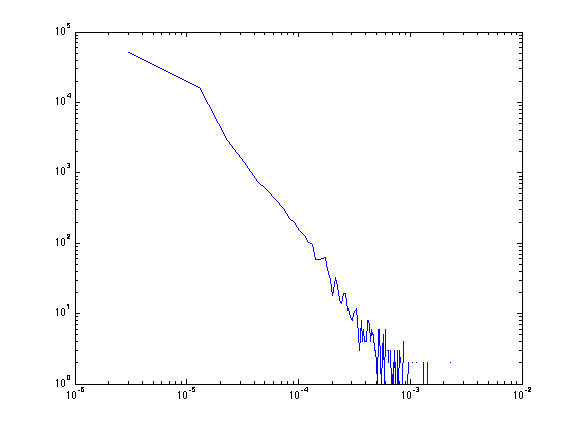
\includegraphics[width=.25\linewidth]{FIG/pagerank/as-skitter_75000.png}}\hfill
\subfloat[ca-AstroPh\label{fig:ca-AstroPh}]
  {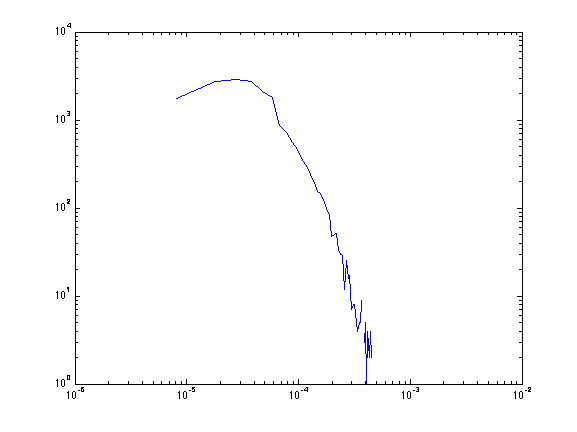
\includegraphics[width=.25\linewidth]{FIG/pagerank/ca-AstroPh.png}}\hfill
\subfloat[cit-HepPh\label{fig:cit-HepPh}]
  {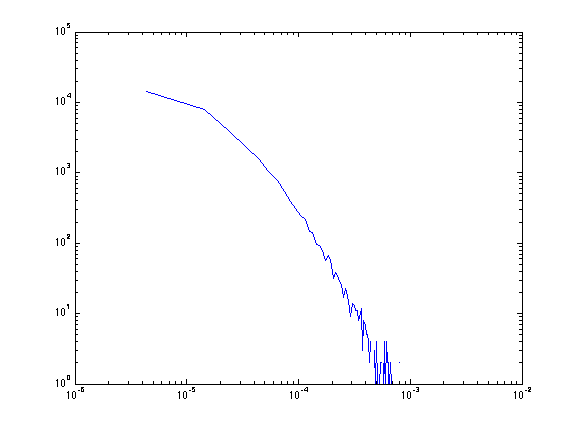
\includegraphics[width=.25\linewidth]{FIG/pagerank/cit-HepPh.png}} \hfill
\subfloat[cit-HepTh\label{fig:cit-HepTh}]
  {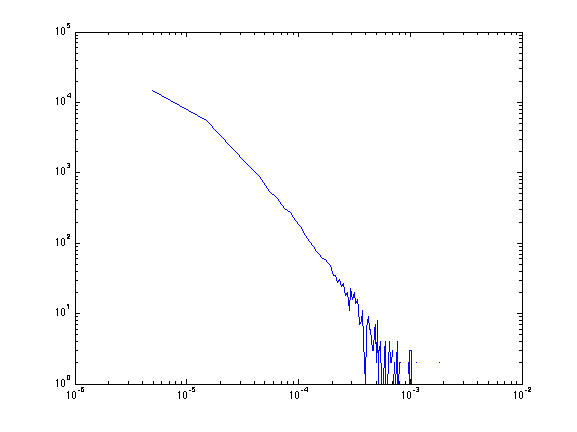
\includegraphics[width=.25\linewidth]{FIG/pagerank/cit-HepTh.png}}\hfill
\subfloat[com-amazon.ungraph-75000\label{fig:com-amazon.ungraph-75000}]
  {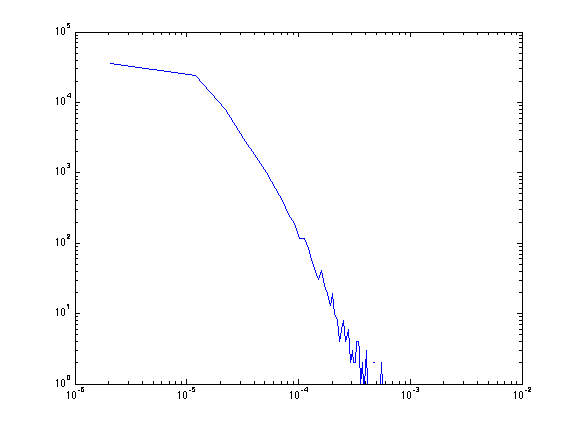
\includegraphics[width=.25\linewidth]{FIG/pagerank/com-amazon.ungraph-75000.png}}\hfill
\subfloat[com-dblp.ungraph-75000\label{fig:com-dblp.ungraph-75000}]
  {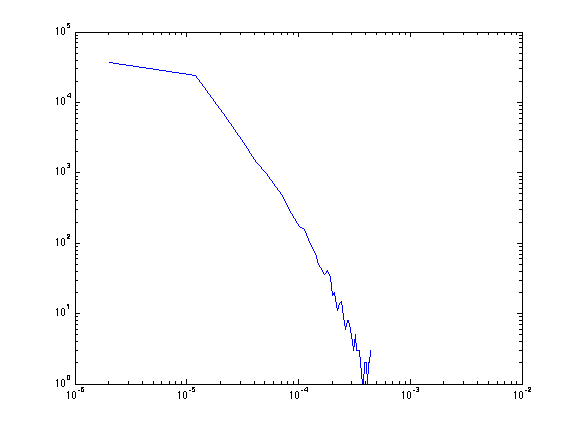
\includegraphics[width=.25\linewidth]{FIG/pagerank/com-dblp.ungraph-75000.png}} \hfill
 \subfloat[email-Enron.ungraph\label{fig:email-Enron.ungraph}]
  {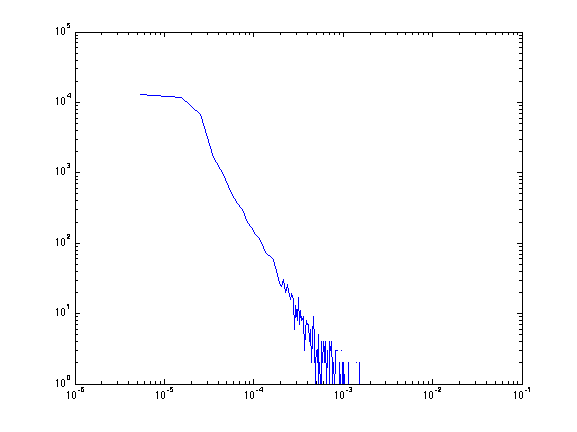
\includegraphics[width=.25\linewidth]{FIG/pagerank/email-Enron.ungraph.png}}\hfill
\subfloat[email-EuAll\label{fig:email-EuAll}]
  {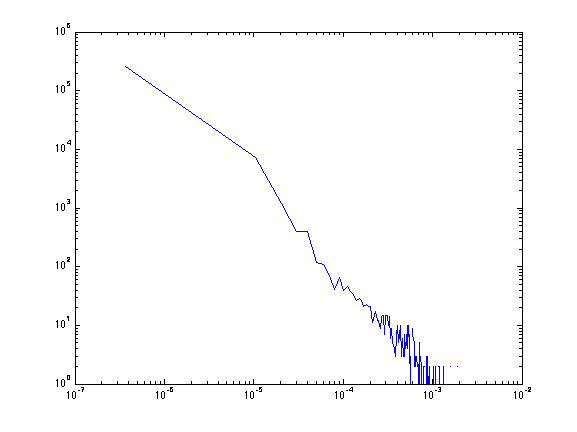
\includegraphics[width=.25\linewidth]{FIG/pagerank/email-EuAll.png}}\hfill
\subfloat[p2p-Gnutella31\label{fig:p2p-Gnutella31}]
  {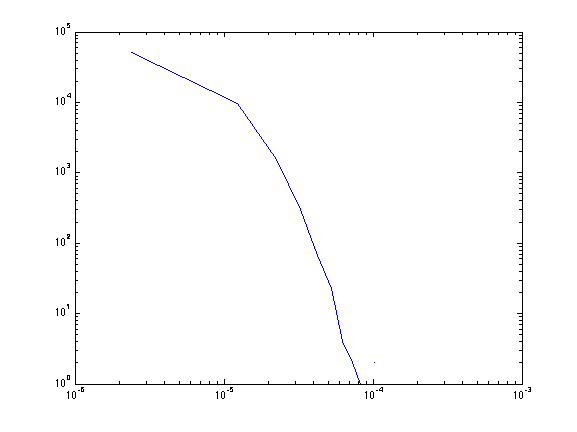
\includegraphics[width=.25\linewidth]{FIG/pagerank/p2p-Gnutella31.png}} \hfill
 \subfloat[soc-Slashdot0811-75000\label{fig:soc-Slashdot0811-75000}]
  {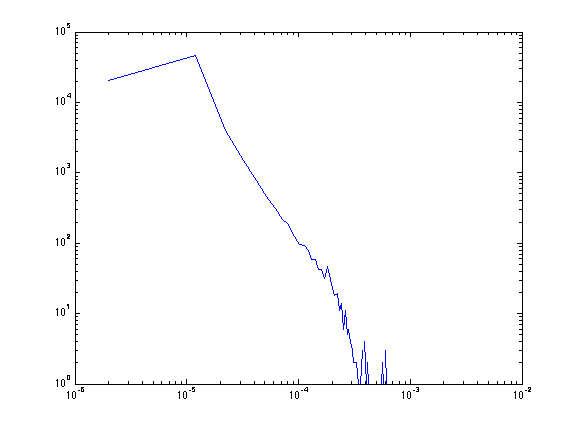
\includegraphics[width=.25\linewidth]{FIG/pagerank/soc-Slashdot0811-75000.png}} 
 \subfloat[as-Caida\label{fig:as-Caida}]
  {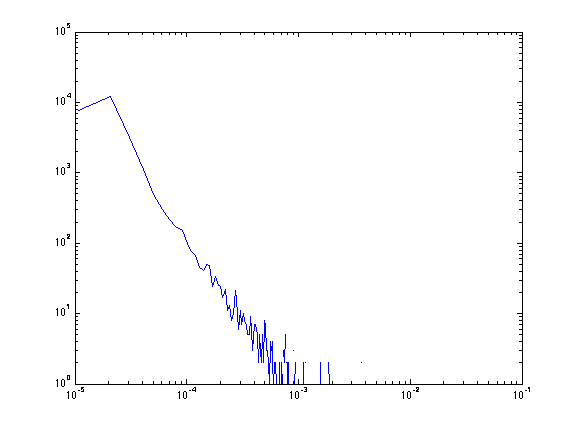
\includegraphics[width=.25\linewidth]{FIG/pagerank/as-Caida.undir.txt.png}} \hfill  
 \subfloat[bio-protein\label{fig:bio-protein}]
  {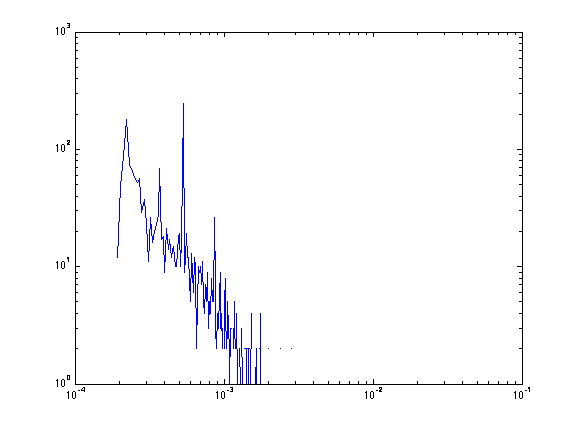
\includegraphics[width=.25\linewidth]{FIG/pagerank/bio-protein-undir.txt.png}} \hfill  
 \subfloat[cit-Cora\label{fig:cit-Cora}]
  {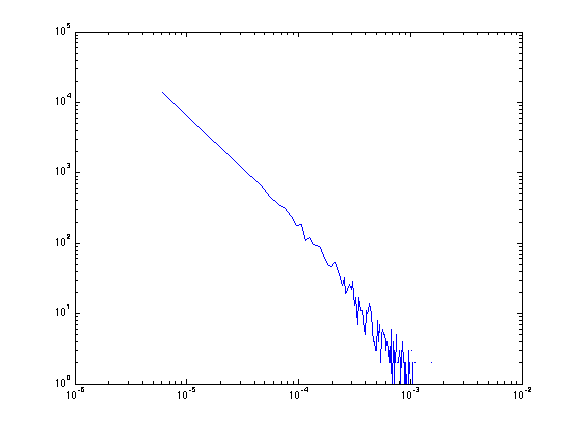
\includegraphics[width=.25\linewidth]{FIG/pagerank/cit-Cora.txt.png}} \hfill 
 \subfloat[soc-digg\label{fig:soc-digg}]
  {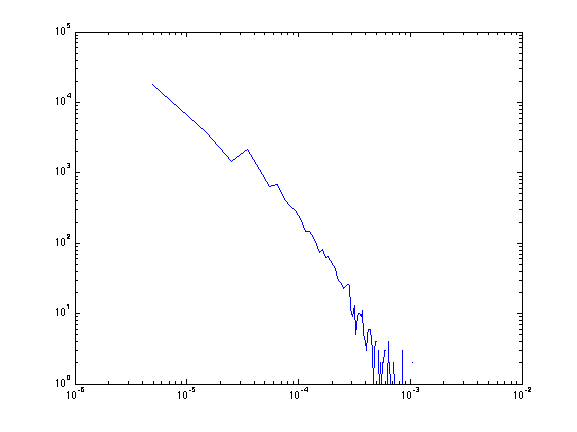
\includegraphics[width=.25\linewidth]{FIG/pagerank/soc-digg.txt.png}} \hfill  
 \subfloat[soc-flickr-75000\label{fig:soc-flickr-75000}]
  {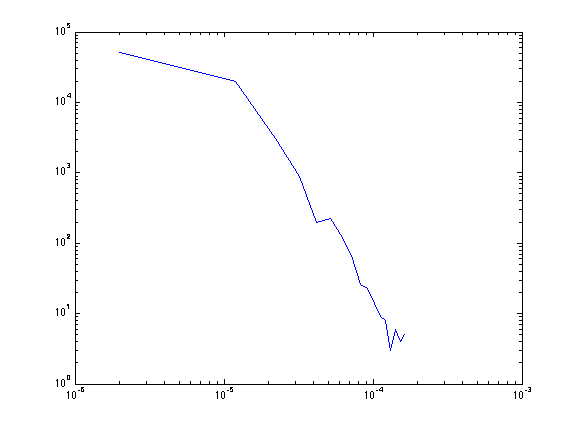
\includegraphics[width=.25\linewidth]{FIG/pagerank/soc-flickr-75000.txt.png}} \hfill  
 \subfloat[soc-hamsterster\label{fig:soc-hamsterster}]
  {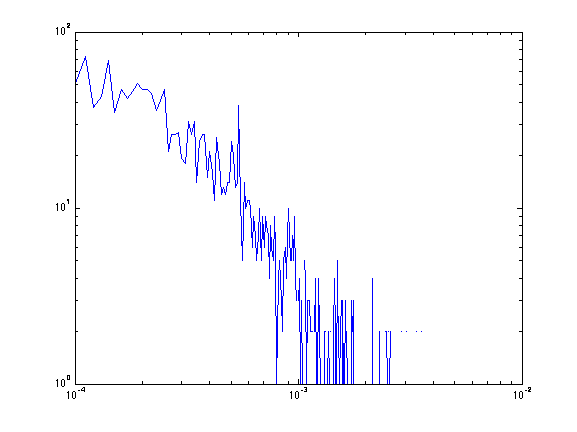
\includegraphics[width=.25\linewidth]{FIG/pagerank/soc-hamsterster.undir.txt.png}} \hfill  
 \subfloat[soc-pokec-75000\label{fig:soc-pokec-75000}]
  {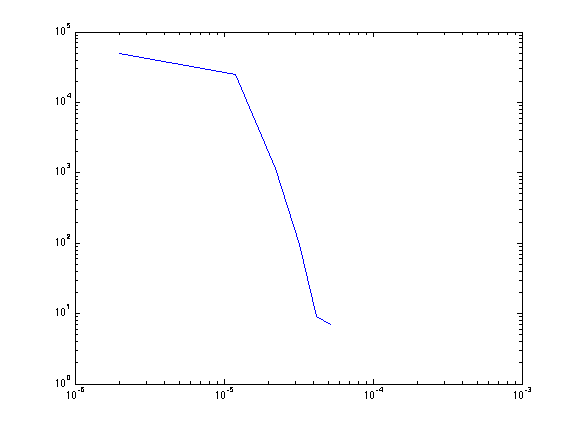
\includegraphics[width=.25\linewidth]{FIG/pagerank/soc-pokec-75000.txt.png}} \hfill  
 \subfloat[soc-Youtube-75000\label{fig:soc-Youtube-75000}]
  {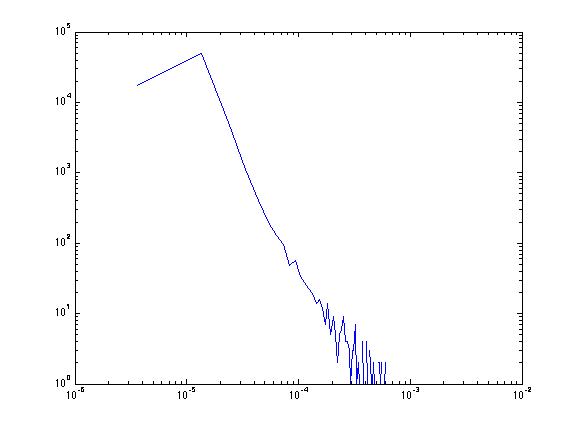
\includegraphics[width=.25\linewidth]{FIG/pagerank/soc-Youtube-75000.undir.txt.png}} \hfill  
 \subfloat[soft-jdkdependency\label{fig:soft-jdkdependency}]
  {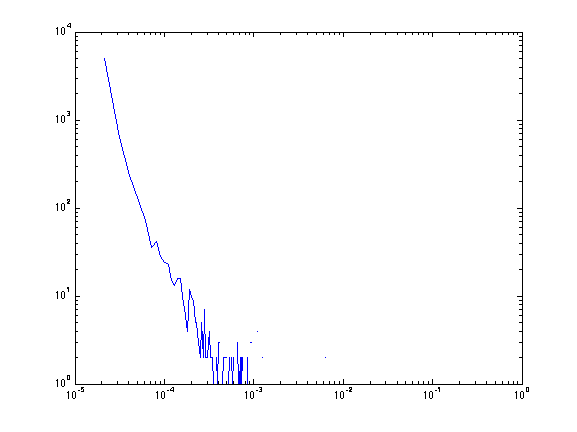
\includegraphics[width=.25\linewidth]{FIG/pagerank/soft-jdkdependency.txt.png}} \hfill  
 \subfloat[text-spanishbook\label{fig:text-spanishbook}]
  {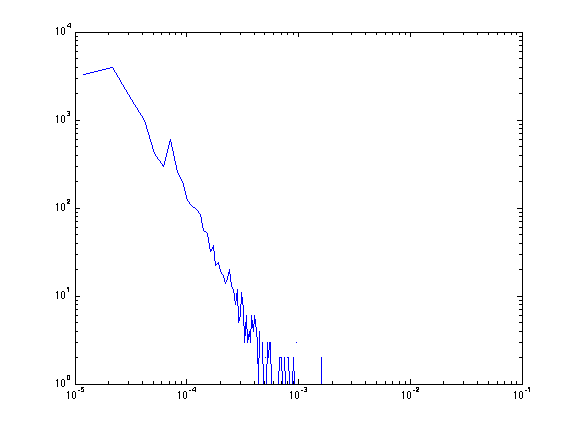
\includegraphics[width=.25\linewidth]{FIG/pagerank/text-spanishbook.txt.png}} \hfill  
\caption{Pagerank value Distributions of 20 graphs}
\label{fig:pagerank}
\end{figure}

To analyze the patterns of PageRank in 20 graphs, we calculated the PageRank value of nodes in each graphs, aggregated the values into distribution, and plotted the distribution in log-log scale. Mainly, we wanted to check whether the distribution of PageRank values follow power law or not. At the same time, we observed the charts of distribution to find out strange patterns of PageRank.
\\
\\
\textbf{Global Pattern}
\\
\\
The experiment result (Figure. \ref{fig:pagerank}) shows that the PageRank value distribution in most of graphs follow power law.
\\
\\
\textbf{Strange Behaviors}
\\
\\
(1) Plateau in the Beginning
\\
\\
The distribution of PageRank in most of graphs follow power low; however, we found that there are plateaus in the beginning part of some distribution charts. Taking com-amazon.ungraph-75000 for example, the line between $10^{-8}$ and $10^{-5}$ is relative smooth. 
\\
ca-AstroPh, com-amazon.ungraph-75000, com-dblp.ungraph-75000, email-Enron.ungraph, soc-Slashdot0811-75000, as-Caida, soc-flickr-75000, soc-pokec-75000, soc-Youtube-75000, and text-spanishbook have such plateau pattern.
\\
\\
(2) Broom Tail
\\
\\
Ideally, the chart of distribution following power law would be a smooth descending straight line in log-log scale plot; however, we found that some lines of real data are not as smooth as ideal straight lines. Instead, the lines of some real data jump up and down in the last part. The shape is like a bloom.
\\
as-skitter, cit-HepTh, email-Enron.ungraph, email-EuAll, as-Caida, cit-Cora, soc-Youtube-75000, soft-jdkdependency, and text-spanishbook have such broom tail pattern.
\\
\\
(3) Vibrating Line
\\
\\
The lines in PageRank distribution chart are usually smooth, but there are some lines vibrating severely. Taking soc-hamsterster for example, its line jumps up and down severely, although the trend of line follow power-law. bio-protein and soc-hamsterster have such pattern.

